\documentclass[a4paper,12pt]{article}

\usepackage[utf8]{inputenc} 
\usepackage[italian]{babel}
\usepackage{indentfirst}
\usepackage[margin=2.2cm]{geometry}
\usepackage[most]{tcolorbox}
\usepackage{graphicx}
\usepackage{subcaption}
\usepackage{hyperref}
\usepackage[italian]{varioref}
\usepackage{listings}
\usepackage{xcolor}
\usepackage[numbered,framed]{matlab-prettifier}
\usepackage[font={small}]{caption}
\usepackage{xcolor}

\usepackage{tikz}
\usetikzlibrary{arrows.meta}
\usetikzlibrary{shapes}
\usetikzlibrary{positioning}
\tikzset{%
  every neuron/.style={
    circle,
    draw,
    minimum size=1cm
  },
  neuron missing/.style={
    draw=none, 
    scale=4,
    text height=0.333cm,
    execute at begin node=\color{black}$\vdots$
  },
}

\captionsetup[figure]{labelfont={bf},name={Figura},labelsep=period}

\renewcommand*{\fullref}[1]{\hyperref[{#1}]{\vref*{#1}, \emph{\nameref*{#1}}}}
\newcommand*{\coderef}[1]{\hyperref[{#1}]{\nameref*{#1} a pagina \pageref*{#1}}}

\renewcommand{\textfraction}{0}
\renewcommand{\topfraction}{1}
\renewcommand{\bottomfraction}{1}
\renewcommand{\floatpagefraction}{1}

\graphicspath{{figures/}}


\title{\textbf{Diagnosi del Diabete}}
\author{Lara Vignotto}
\date{\today}  


\begin{document}

\maketitle

\vfill
\tableofcontents


%%%%%%%%%%%%%%%%%%%%%%%%%%%%%%
\newpage
\section{Presentazione e scopi del progetto} % cap1

Lo scopo di questo progetto è la progettazione e l'implementazione di una rete neurale multistrato in grado di prevedere (classificare) il risultato di un test a partire da dei dati clinici. La rete neurale, idealmente, potrebbe essere utilizzata come strumento a supporto della diagnosi di diabete. 
\begin{itemize}
  \item Nel \textbf{secondo capitolo} presenteremo le specifiche del modello di rete neurale adottato e l'architettura che ne deriva;
  \item Nel \textbf{terzo capitolo} daremo una panoramica sulla struttura del software, espondendo i moduli che compongono il pacchetto;
  \item Nel \textbf{quarto capitolo} riporteremo il codice con alcuni commenti e precisazioni;
  \item Nel \textbf{quinto capitolo} presenteremo i risultati;
  \item Nell'\textbf{settimo capitolo} discuteremo i risultati mostrati al capitolo precedente.
\end{itemize}



%%%%%%%%%%%%%%%%%%%%%%%%%%%%%%
\newpage
\section{Modello e architettura della rete} % cap2

La rete neurale è composta da quattro strati (Figura~\vref{fig:modello}):
\begin{itemize}
    \item Un \emph{input layer} di 8 nodi, che corrispondono agli otto dati clinici rilevati dai pazienti;
    \item Due \emph{hidden layers} di 40 nodi con funzione di attivazione sigmoide;
    \item Un \emph{output layer} di 1 nodo (positivo/negativo) con funzione di attivazione sigmoide.
\end{itemize}

\begin{figure}[htb]
  \center
  \tcbox[boxrule=.3mm,colback=white]{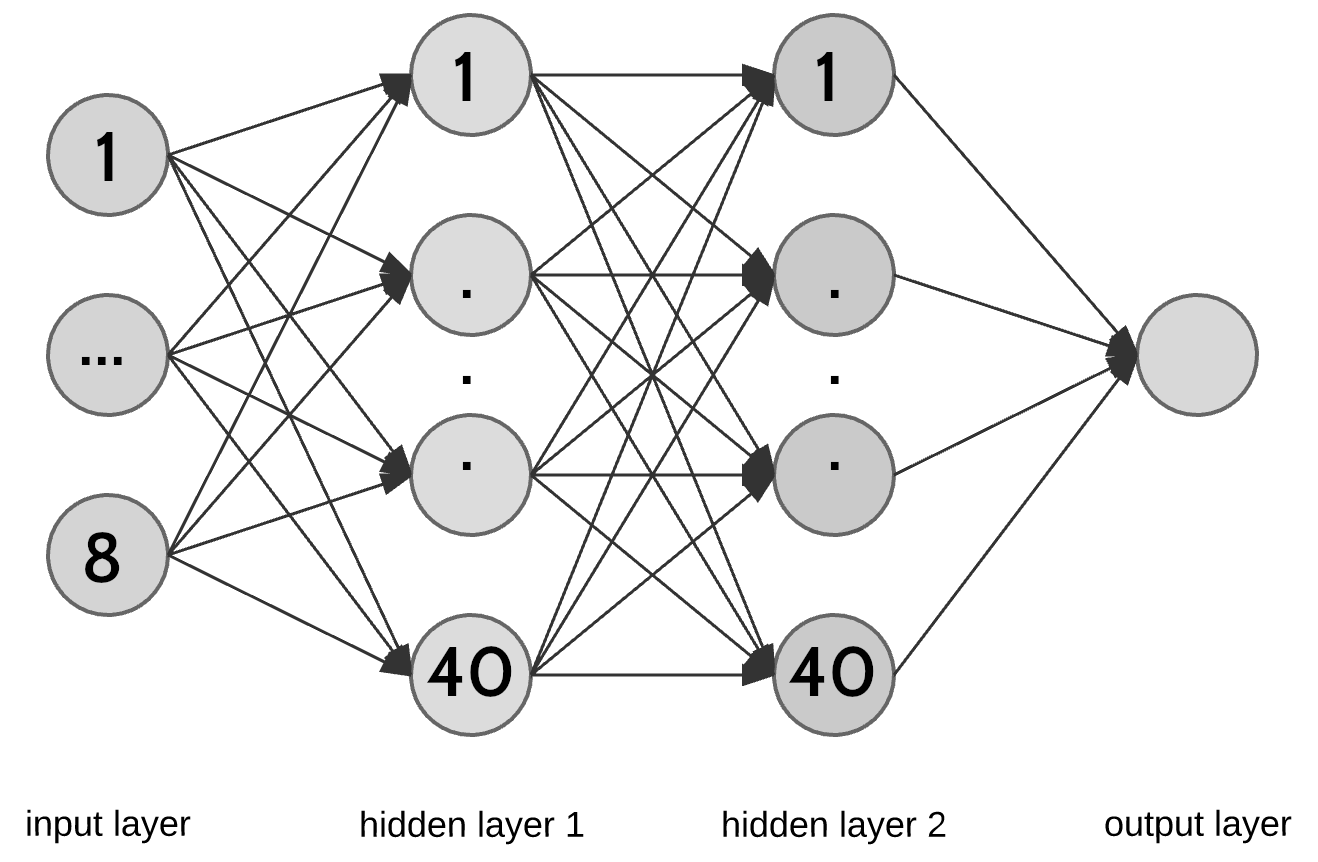
\includegraphics[width=.9\textwidth]{modello.png}}
  \caption{Schema della rete neurale.}
  \label{fig:modello}
\end{figure}



%%%%%%%%%%%%%%%%%%%%%%%%%%%%%%
\newpage
\section{Struttura del software} % cap3

Il pacchetto per questa rete neurale è composto da quattro moduli, ovvero 1 script e 3 funzioni:
\begin{itemize}
    \item La funzione \texttt{Diabetes\_DataPrep} per la preparazione dei dati;
    \item Lo script \texttt{Diabetes\_Training} per la definizione dell'architettura di rete, l'impostazione dell'apprendimento e la valutazione di prestazioni;
    \item La funzione \texttt{Diabetes\_DeltaRule} che applica la regola di apprendimento;
    \item La funzione di attivazione \texttt{Sigmoid}.
\end{itemize}

\begin{figure}[htb]
  \centering
  \tcbox[boxrule=.3mm,colback=white]{
\begin{tikzpicture}
  \node (c) [xshift=8cm,yshift=-1cm,draw,draw,rectangle,rounded corners] 
  {\texttt{Sigmoid}};
  \node (e) [xshift=1.5cm,yshift=-3cm,draw,rectangle,rounded corners] 
  {\texttt{Diabetes\_DataPrep}};
  \node (f) [xshift=8cm,yshift=-3cm,draw,rectangle,rounded corners] 
  {\texttt{Diabetes\_DeltaRule}};
  \node (g) [xshift=4.5cm,yshift=-5cm,draw,rectangle,rounded corners] 
  {\texttt{Diabetes\_Training}};

  \draw   [-{Latex[length=3mm]}] (c)--(f);
  \draw   [-{Latex[length=3mm]}] (e)--(g);
  \draw   [-{Latex[length=3mm]}] (f)--(g);
\end{tikzpicture}
  }
  \caption{Schema dei moduli software e legami tra loro.}
  \label{fig:schema-software}
\end{figure}



%%%%%%%%%%%%%%%%%%%%%%%%%%%%%%
\newpage
\section{Codice} % cap4


\begin{lstlisting}[style=Matlab-editor,title=\texttt{Diabetes\_DataPrep.m},label=lst:dataprep]
function [TrainingData, TrainingLabels, ValidationData, ... 
    ValidationLabels] = Diabetes_DataPrep()
%
    DataSet = readmatrix('diabetes.csv');
%
%%%%%%%%%%%%%%%%%%% Splitting
%   Numero totale dei campioni
    numtotData = 768;
%	  Percentuale di splitting
    training_perc = 0.8; 
%
%	  Randomizzazione degli indici delle immagini
    split_perm = randperm(numtotData);
%
%	  Cardinalita' dell'insieme di apprendimento (training)
    training_cardin = floor(numtotData * training_perc);
%
%	  Definizione degli insiemi di apprendimento 
%	  e delle relative etichette, tutti randomizzati;
    TrainingData = DataSet(split_perm(1:training_cardin),1:8);
    TrainingLabels = DataSet(split_perm(1:training_cardin),9);
%
%	  Definizione degli insiemi di collaudo 
%	  e delle relative etichette, tutti randomizzati
    ValidationData = ... 
        DataSet(split_perm(training_cardin+1:end),1:8);
    ValidationLabels = ... 
        DataSet(split_perm(training_cardin+1:end),9);
end
\end{lstlisting}


\newpage
\begin{lstlisting}[style=Matlab-editor,title=\texttt{Diabetes\_Training.m},label=lst:training]
alpha = 0.01;
%
[TrainingData, TrainingLabels, ValidationData, ... 
    ValidationLabels] = Diabetes_DataPrep();
%
% Inizializzazione casuale dei pesi
w1 = 2 * rand(40, 8) - 1;   % input > hidden1
w2 = 2 * rand(40, 40) - 1;  % hidden1 > hidden2
w3 = 2 * rand(1, 40) - 1;   % hidden2 > output
%
% Iperparametro col numero di epoche
N_epoch = 150;
%
% Inizializzazione dei vettori per i grafici
MSE_Train = []; % MSE per epoca (apprendimento)
epoch0 = [];    % epoche
%
% Inizia il ciclo di apprendimento sulle epoche
for epoch = 1:N_epoch
%
    [w1, w2, w3, output_matrix] = ...
        Diabetes_DeltaRule(w1, w2, w3, TrainingData, ... 
        TrainingLabels, alpha);
%
%   Concatena l'epoca corrente al vettore delle epoche
    epoch0 = [epoch0 epoch];
%
%   Concatena l'MSE_Learn osservato in fase di apprendimento
%   sullo strato di output per l'epoca corrente
    MSE_T = immse(output_matrix, TrainingLabels);
    MSE_Train = [MSE_Train MSE_T];
%
end % fine ciclo sulle epoche
%
% Grafico della curva di apprendimento 
plot(epoch0(1:150),MSE_Train(1:150),'LineWidth',3), grid;
title('Learning Curve (Loss)')
xlabel('epoch')
ylabel('MSE Train')
hold on
%
% Memorizzazione su file dei valori dei pesi cosi' calcolati
save('Diabetes_Trained_Network.mat');
\end{lstlisting}



\newpage
\begin{lstlisting}[style=Matlab-editor,title=\texttt{Diabetes\_DeltaRule.m},label=lst:deltarule]
function [w1, w2, w3, output_matrix] = ...
    Diabetes_DeltaRule(w1, w2, w3, input_data, correct_output, alpha)
%
%%%%%%%%%%%%%%% Settaggio dei parametri
%
    N = 614; % numero dei dati
%
%%%%%%%%%%%%%%% Ciclo sui dati di input
%%%%%%%%%%%%%%%%%%%
    for k = 1:N
%       Trasposta della matrice di input
        input_data_transposed = input_data';
        correct_input_data = input_data_transposed(:,k);
%
%%%%%%%%%%%%%%% Inizia la fase di feedforward
%
%       Trasmissione attivazione dallo strato di input a
%       hidden1
        input_to_hidden_layer1 = w1*correct_input_data;
        output_of_hidden_layer1 = ... 
            Sigmoid(input_to_hidden_layer1);
%
%       Trasmissione attivazione da hidden1 a hidden2
        input_to_hidden_layer2 = w2*output_of_hidden_layer1;
        output_of_hidden_layer2 = ... 
            Sigmoid(input_to_hidden_layer2);
%
%       Trasmissione attivazione da hidden2
%       allo strato di output
        input_to_output_node = w3*output_of_hidden_layer2;
%
%       Normalizzazione dei valori di output tramite Sigmoid
        final_output = Sigmoid(input_to_output_node);
%
%       Calcolo della trasposta del correct_output
        correct_output_transpose = correct_output(k, :)';
%
%       Calcolo dell'errore sullo strato di output
        error = correct_output_transpose - final_output;
%
%%%%%%%%%%%%%%% Fase di backpropagation
%       Calcolo della delta rule
        delta = error;
%
        error_of_hidden_layer2 = w3'*delta;
        delta2=(input_to_hidden_layer2>0) .* ... 
            error_of_hidden_layer2;
%
        error_of_hidden_layer1 = w2'*delta2;
        delta1=(input_to_hidden_layer1>0) .* ... 
            error_of_hidden_layer1;
%
%       Calcolo dell'aggiornamento dei pesi tramite delta rule
        update_of_w3 = alpha*delta*output_of_hidden_layer2';
        update_of_w2 = alpha*delta2*output_of_hidden_layer1';
        update_of_w1 = alpha*delta1*correct_input_data';
%
%       Aggiornamento delle matrici dei pesi
        w1 = w1 + update_of_w1;
        w2 = w2 + update_of_w2;
        w3 = w3 + update_of_w3;
%
%       Aggiornamento della matrice degli output
        output_matrix(k,:) = final_output';
%
    end % fine ciclo sulle cifre
%
end % fine function
\end{lstlisting}



\vfill
\begin{lstlisting}[style=Matlab-editor,title=\texttt{Sigmoid.m},label=lst:sigmoid]
function y = Sigmoid(x)
    y = 1./(1+exp(-x));
end
\end{lstlisting}



%%%%%%%%%%%%%%%%%%%%%%%%%%%%%%
\newpage
\section{Risultati} % cap risultati

Durante la procedura di apprendimento abbiamo calcolato e raccolto i dati necessari a tracciare delle curve \emph{loss}. Il \emph{learning rate} è stato impostato ad un valore di 0.01, mentre il numero di epoche a 150. I grafici risultanti sono nelle Figure~\vref{fig:loss1}, \vref{fig:loss2} e \vref{fig:loss3}.

\begin{figure}[htb]
  \center
  \tcbox[boxrule=.3mm,colback=white]{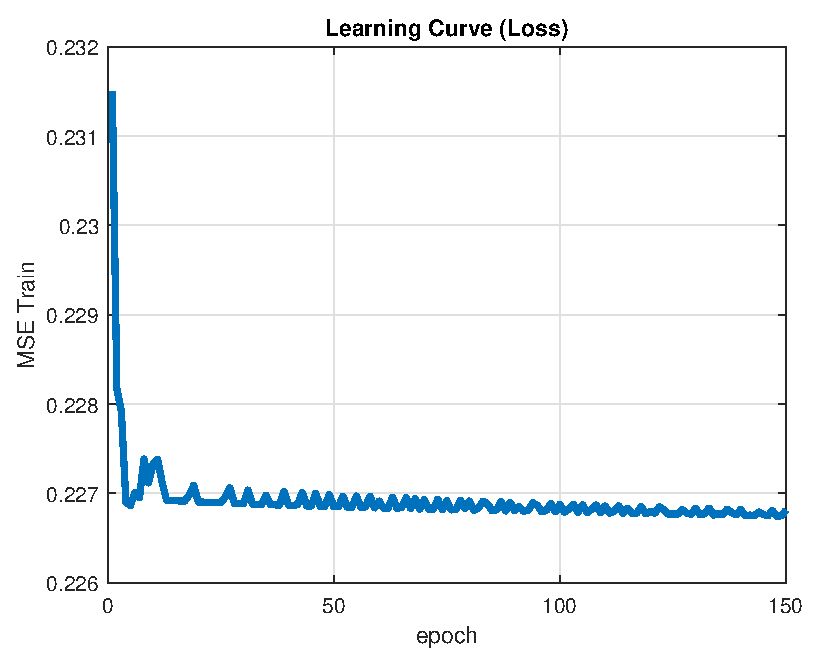
\includegraphics[width=.8\textwidth]{loss-curve.eps}}
  \caption{Curva loss (1).}
  \label{fig:loss1}
\end{figure}


\begin{figure}[htp]
  \centering
  \tcbox[boxrule=.3mm,colback=white]{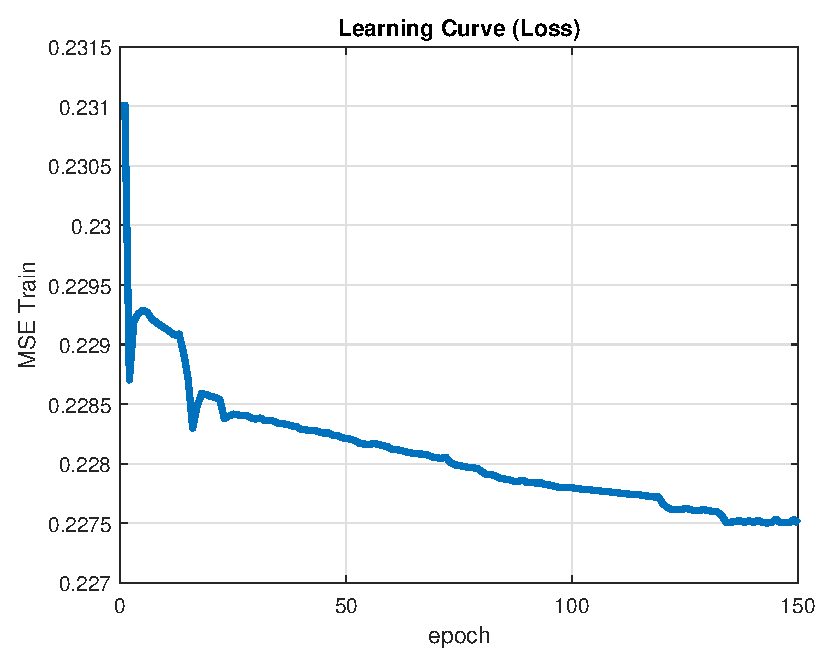
\includegraphics[width=.8\textwidth]{loss-curve2.eps}}

  \medskip

  \tcbox[boxrule=.3mm,colback=white]{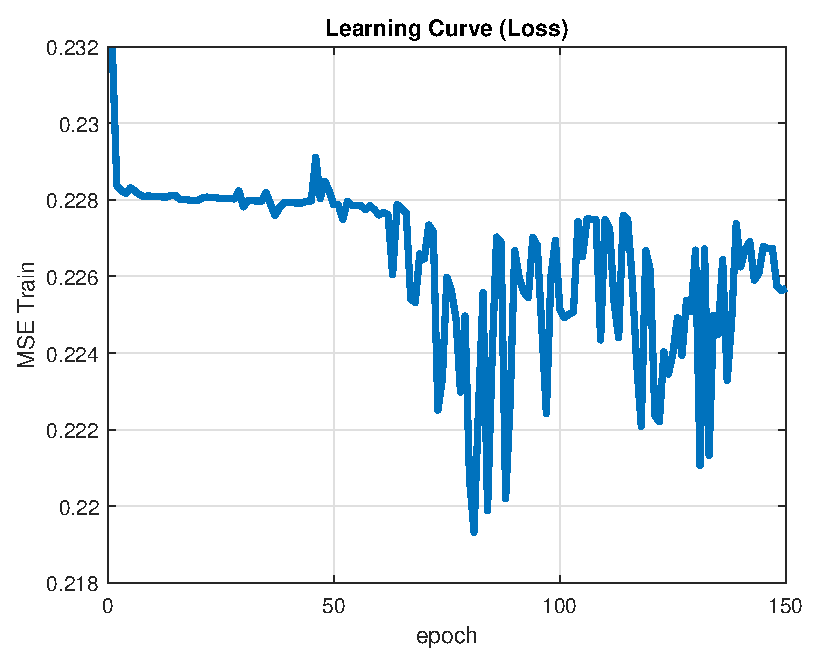
\includegraphics[width=.8\textwidth]{loss-curve3.eps}}

  \caption{Curve loss (2--3).}
  \label{fig:loss2}
\end{figure}


\begin{figure}[htp]
  \centering
  \tcbox[boxrule=.3mm,colback=white]{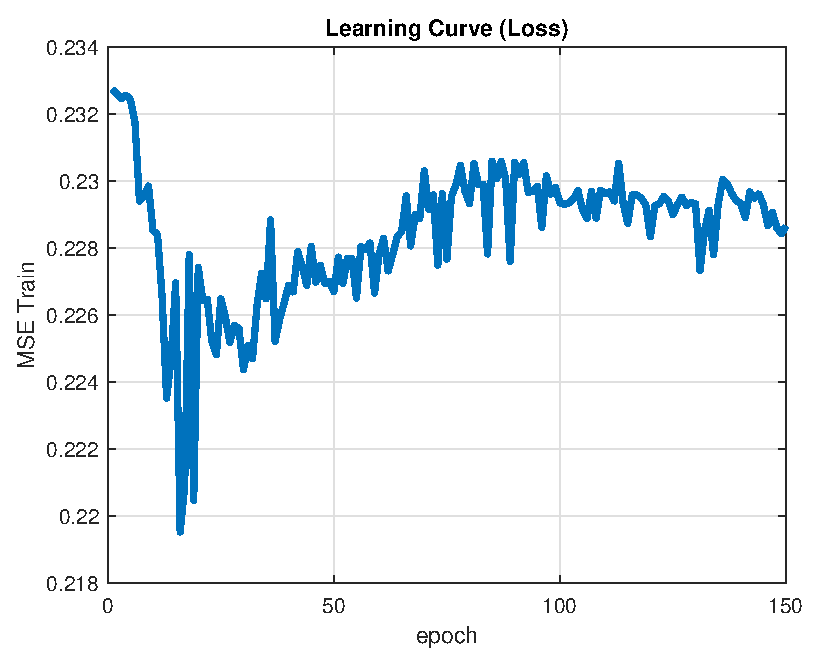
\includegraphics[width=.8\textwidth]{loss-curve4.eps}}

  \medskip

  \tcbox[boxrule=.3mm,colback=white]{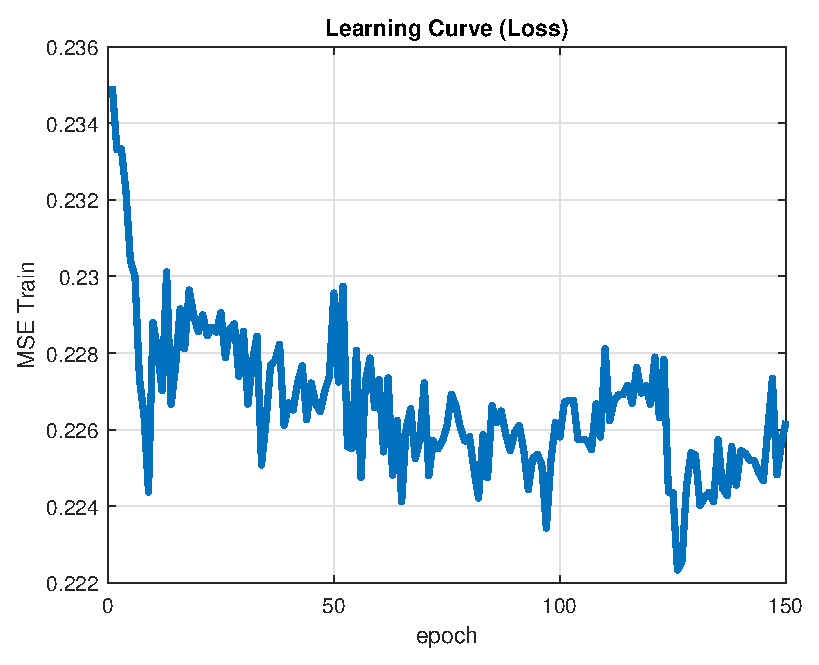
\includegraphics[width=.8\textwidth]{loss-curve5.eps}}

  \caption{Curve loss (4--5).}
  \label{fig:loss3}
\end{figure}



%%%%%%%%%%%%%%%%%%%%%%%%%%%%%%
\newpage
\section{Osservazioni e Conclusioni} % cap conclusioni

Abbiamo addestrato la rete utilizzando un \emph{training set} di 614 elementi scelti a caso dall'intero dataset, e un valore di tasso di apprendimento pari a $0.01$. Durante l'apprendimento, ad ogni epoca abbiamo calcolato il \emph{mean squared error} tra l'\emph{output} della rete e il valore corretto. Con questi dati abbiamo tracciato la curva \emph{loss}.

Possiamo osservare come le curve di apprendimento non tendano sempre a diminuire. In particolare, anche quelle che diminuiscono presentano delle intabilità. Queste potrebbero essere spiegate dall'effetto di saturazione, ovvero che per effetti numerici l'MSE non converge. 

Inoltre notiamo come il valore proprio dell'MSE è piuttosto alto: si aggira attorno a 0.22 nei suoi picchi minimi.

\paragraph{Alternative implementative.} Per migliorare la stabilità della rete e la sua capacità di previsione, si potrebbe modificare il \emph{learning rate} (ad esempio 0.1) e il numero di epoche (aumentandole). Inoltre, si potrebbero utilizzare delle funzioni di attivazione diverse. Questo verrebbe fatto per cercare di diminuire il più possibile l'errore. 

Alternativamente, si potrebbe definire l'architettura di rete utilizzando il toolbox \texttt{layers} di Matlab.

Un test che potrebbe essere fatto è quello dell'accuratezza, utilizzando il \emph{validation set}. Applicando nuovamente una fase di \emph{feedforward} sulla rete addestrata si potrebbe calcolare la percentuale di \emph{samples} classificati correttamente.





\end{document}